\begin{figure*}[htb]
    \centering
    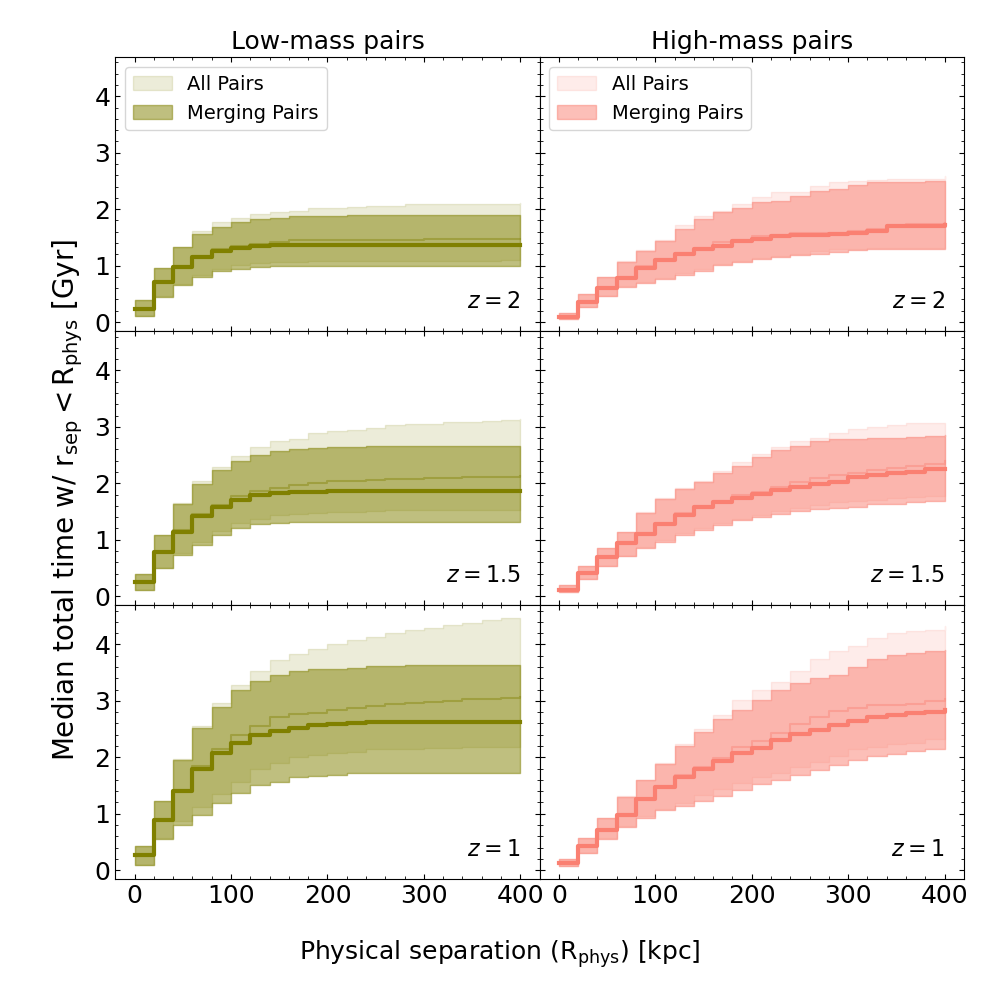
\includegraphics[width=\textwidth]{plots/bet-on-it/2_medtotal_LoHi.png}
    \caption{\kc{reverse the direction of z} 
    The median (solid) and 1st-3rd quartile spread (shaded regions) of the cumulative time that isolated low-mass pairs (left) and high-mass pairs (right) spend with separations \rsep{} between $10\kpc$ and \Rphys{}. 
    The Merging Pairs sample (dark green and dark pink) selected at $z=(1,1.5,2)$ merge before $z=0$, while the All Pairs sample (light green and light pink) include all the pairs from the \paircat{} (mergers and non-mergers).  
    The low-mass (high-mass) merging pairs represent XX\%(XX\%) of the low-mass (high-mass) pair sample at $z=1,1.5, \mbox{and } 2$ respectively. 
    The sample of All Pairs spend more time at higher separations than the merging pairs, as expected since the non-merging pairs are not likely to have very low separations that would result in mergers prior to $z=0$. 
    For a more direct comparison between the low-mass and high-mass pairs, see Fig.~\ref{fig:phys-vs-scaled}. 
    }
    \label{fig:low-vs-high}
\end{figure*}

% \begin{figure*}[htb]
%     \centering
%     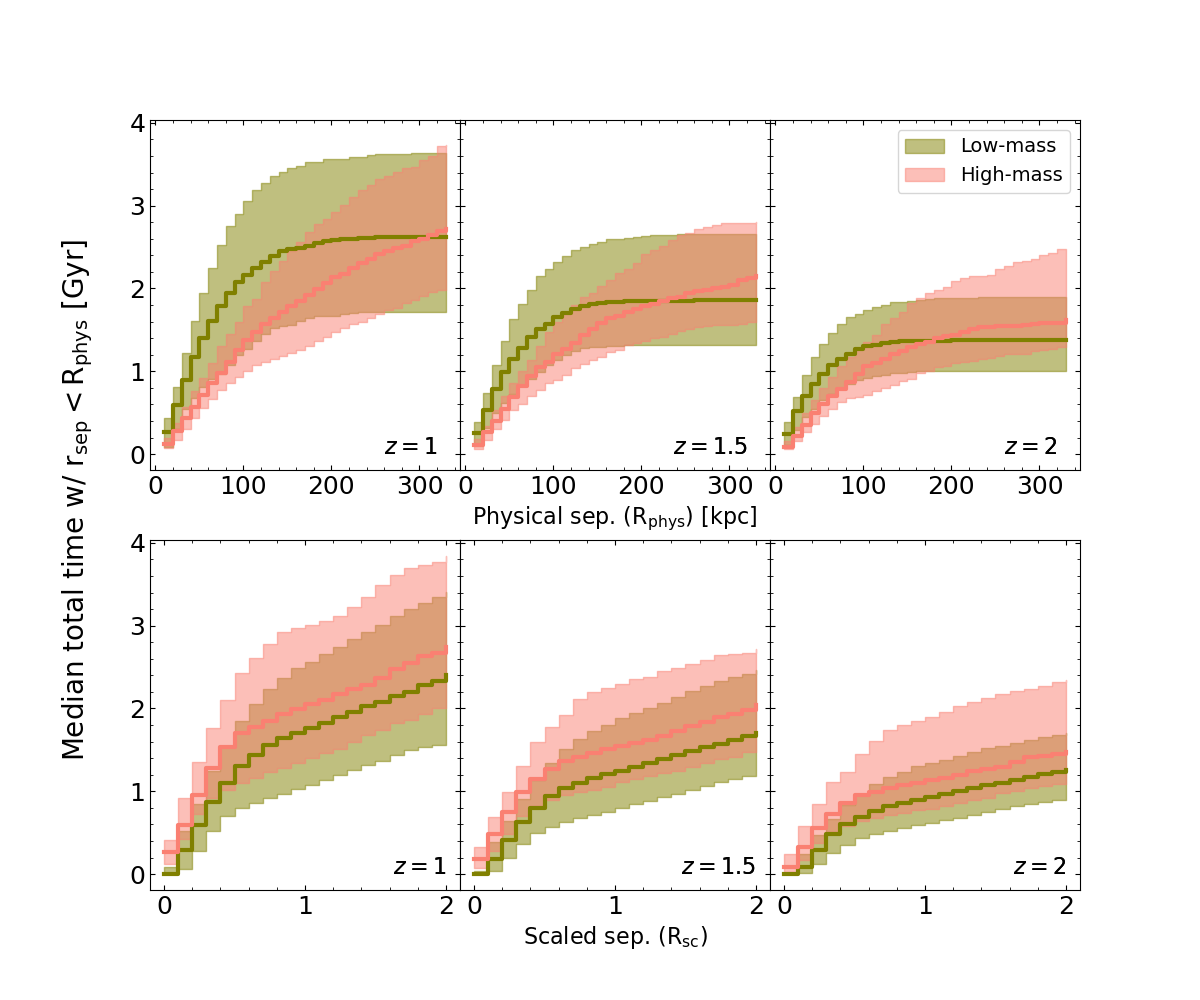
\includegraphics[width=\textwidth]{plots/bet-on-it/2_medtotal_PhScT.png}
%     \caption{\kc{Add legend to plot, and I think reverse the direction of z} 
%     The median and 1st-3rd quartile spread of the cumulative time that isolated merging pairs, selected at $z=(1,1.5,2)$, spend with separations \rsep{} greater than $10\kpc$ and less than either \Rphys{} or \Rsc{}.
%     %
%     (Top) The median total time spent by isolated merging pairs with separations between $10\kpc$ and \Rphys{}.
%     Low-mass pairs spend a longer amount of time within $\sim200\kpc$ than high-mass pairs at each of these redshifts. 
%     However, high-mass galaxies spend more time at higher separations of $\rsep>200-300\kpc$. This is because the elapsed time is measured starting at the infall snapshot of the pair, and high-mass halos have larger radii, the high-mass halo orbits have a broader distribution of separations that extend to larger separations than those of the low-mass pairs.
%     (Bottom) The median total time spent by pairs with separations greater than $\rsep>10\kpc$ and less than a given fraction of the virial radius ($\rsep/\Rvir<\Rsc$) of the pair, which scales with mass and redshift.  
%     High-mass pairs spend more time within the same scaled separation than low-mass pairs. For example, a high-mass pair selected from the $z=1.5$ sample will spend \kc{XXGyr} within \kc{$1\Rsc\sim XX\kpc$}, while a low-mass pair from the same sample will spend \kc{XXGyr} within \kc{$1\Rsc\sim XX\kpc$}. 
%     Low-mass and high-mass pairs have similar cumulative time profiles as a function of scaled separation, with a roughly constant offset for all scaled separations. 
%     The high-mass pairs spend a median of \kc{$XX\Gyr$} more than low-mass pairs at every scaled separation at $z=1$ and $z=1.5$, and a median of \kc{$XX\Gyr$} more $z=2$.
%     }
%     \label{fig:phys-vs-scaled}
% \end{figure*}


% \begin{figure*}[htb]
%     \centering
%     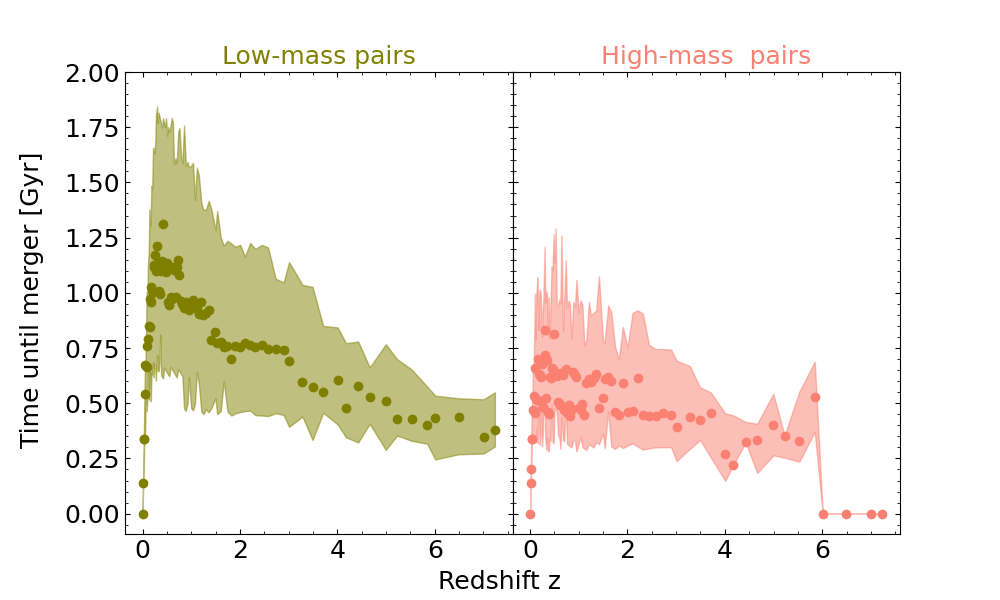
\includegraphics[width=\textwidth]{plots/bet-on-it/3_Timevsz.png}
%     \caption{}
%     % \label{fig:low-vs-high}
% \end{figure*}
% \begin{figure*}[htb]
%     \centering
%     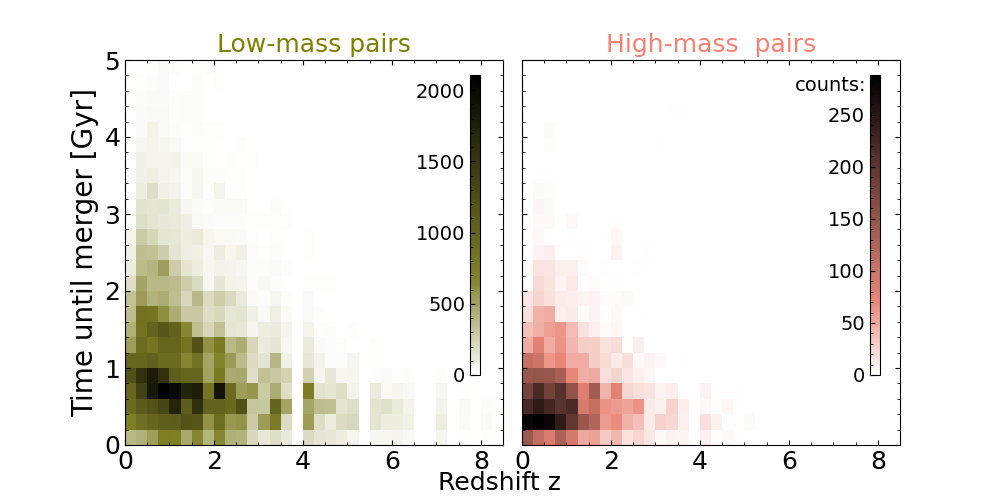
\includegraphics[width=\textwidth]{plots/bet-on-it/3_Timevsz-2d.png}
%     \caption{}
%     % \label{fig:low-vs-high}
% \end{figure*}


% \begin{figure}[htb]
%     \centering
%     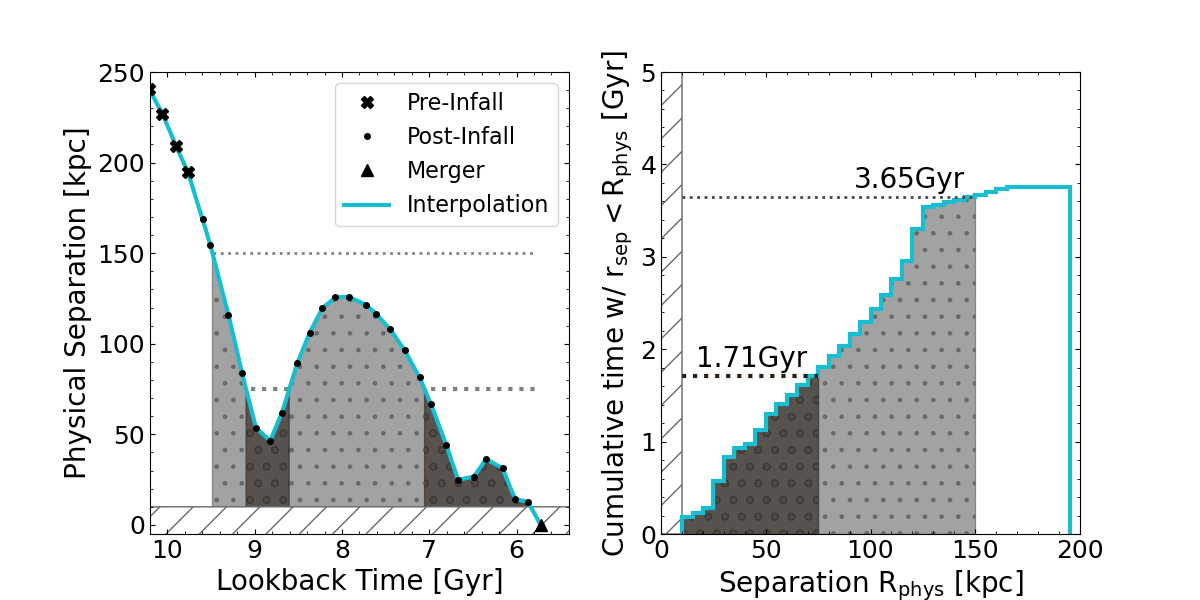
\includegraphics[width=0.5\columnwidth]{plots/bet-on-it/4_example1.png}
% \end{figure}
% \begin{figure}[htb]
%     \centering
%     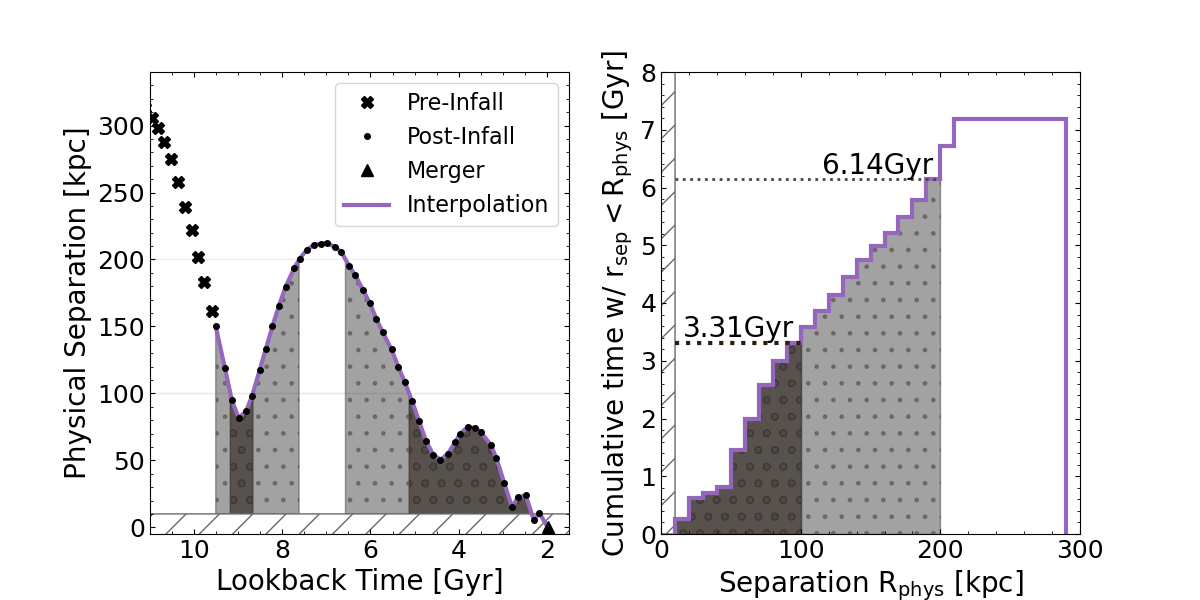
\includegraphics[width=0.5\columnwidth]{plots/bet-on-it/4_example2.png}
%     \caption{}
% \end{figure}
% \begin{figure}[htb]
%     \centering
%     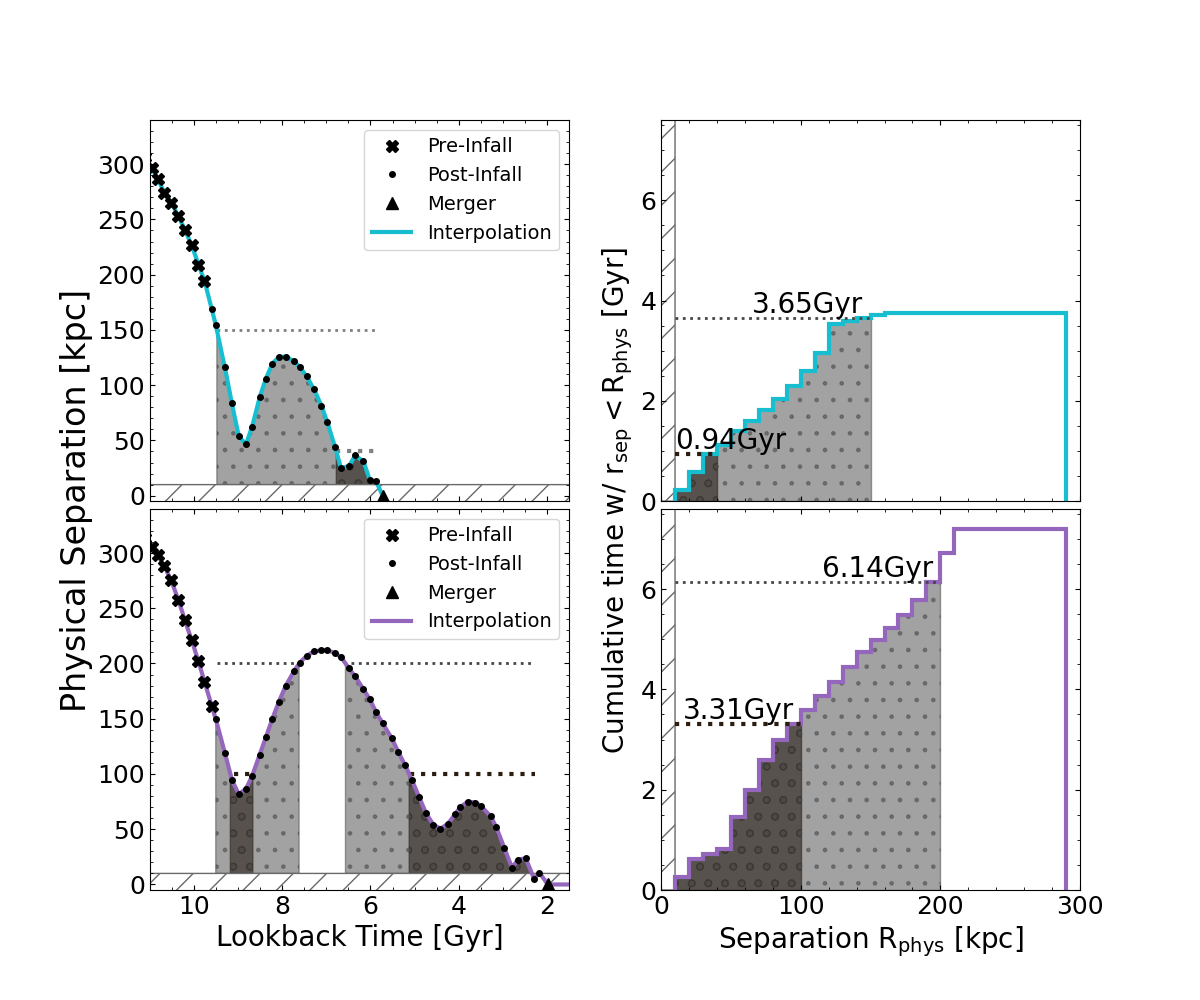
\includegraphics[width=0.5\columnwidth]{plots/bet-on-it/4_examplecombo.png}
% \end{figure}

% \begin{figure}[htb]
%     \centering
%     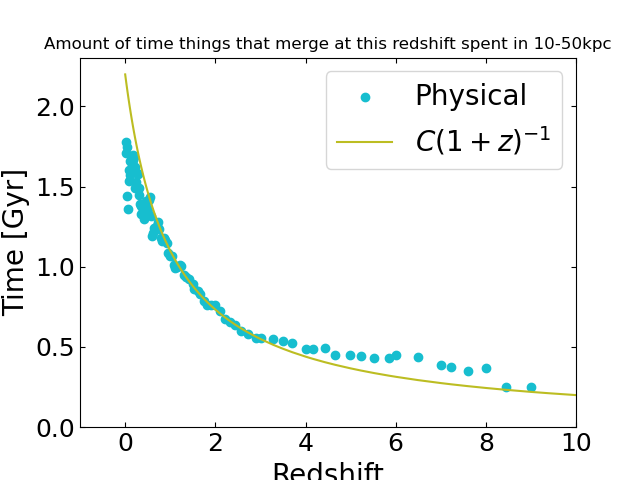
\includegraphics[width=0.5\columnwidth]{plots/bet-on-it/3_timeinbin_beforemerger.png}
% \end{figure}
% \begin{figure}[htb]
%     \centering
%     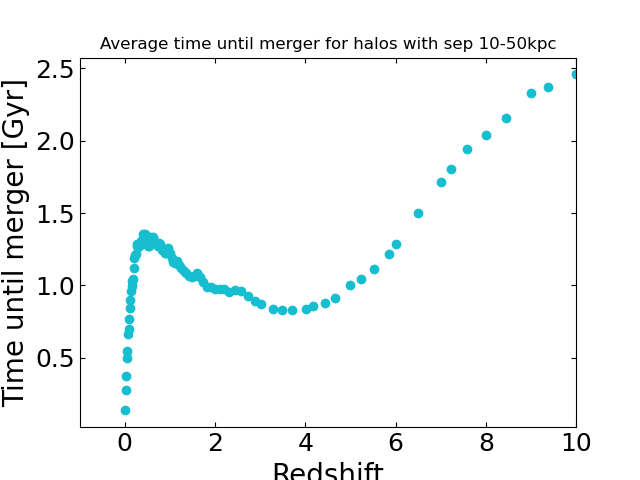
\includegraphics[width=0.5\columnwidth]{plots/bet-on-it/3_timeinbin_untilmerger_phys.png}
% \end{figure}

% \begin{figure*}[htb]
%     \centering
%     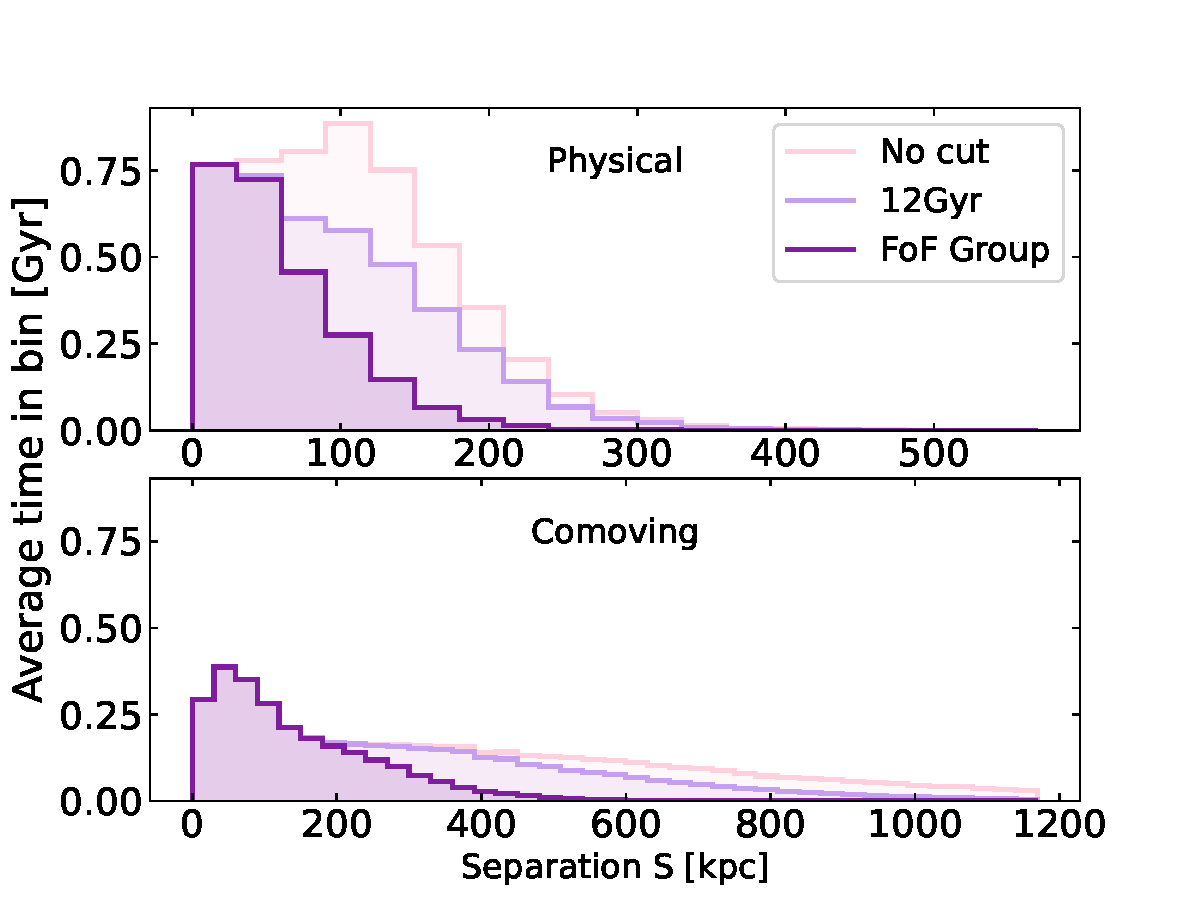
\includegraphics[width=\columnwidth]{plots/4_timescales/timevssep_phys+co.pdf}
%     \caption{}
%     % \label{fig:phys-comoving}
% \end{figure*}

% \begin{figure*}[htb]
%     \centering
%     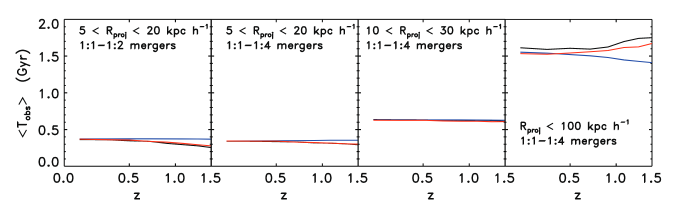
\includegraphics[width=\columnwidth]{lotz.png}
%     \caption{}
%     % \label{fig:phys-comoving}
% \end{figure*}